\documentclass[letterpaper]{article}
\usepackage[dvipsnames]{xcolor}
\usepackage{tikz,amsmath,amssymb}
\usetikzlibrary{decorations.text}
\begin{document}
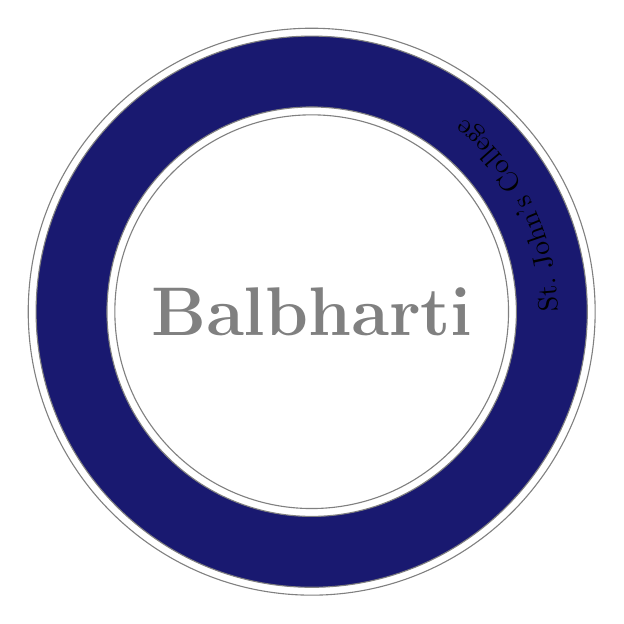
\begin{tikzpicture}
\begin{scope}
\draw[color=gray,fill=MidnightBlue] (0,0) circle (3.5cm);
\draw[color=gray,fill=white] (0,0) circle (2.6cm);
\end{scope}
\draw[color=gray] (0,0) circle (2.5cm) node {\Huge\bf Balbharti};
\draw[color=gray] (0,0) circle (3.6cm);
\path [postaction={decorate,decoration={raise=-2pt,text along path, 
text=St. John's College}}] (0,0) circle (3.05cm);
\end{tikzpicture}
\end{document}